\section{Elektromagnetiskt fält}

\begin{wrapfigure}[8]{R}{0.5\textwidth}
  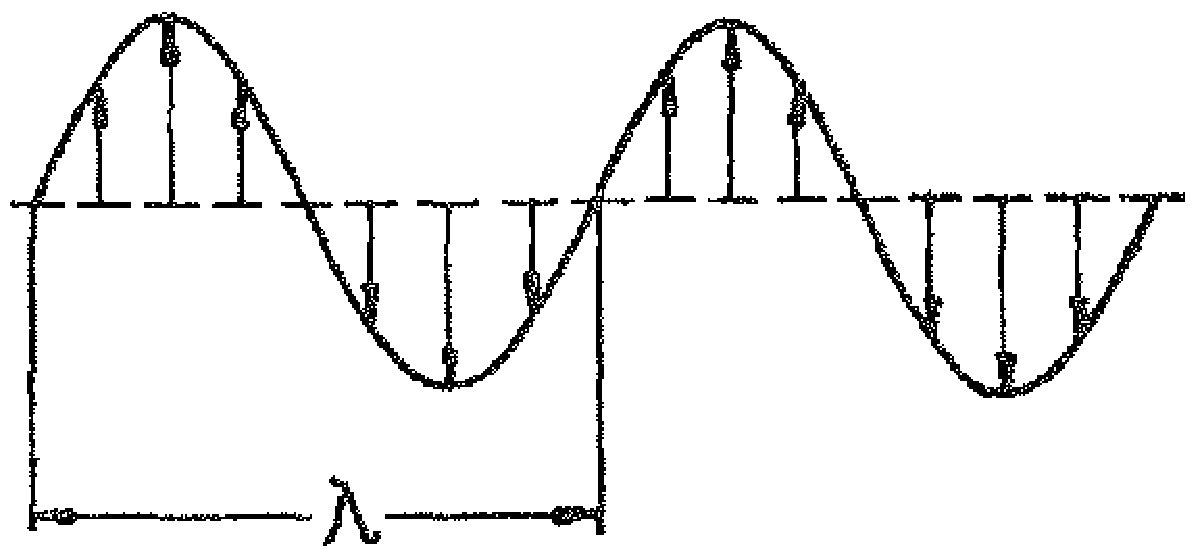
\includegraphics[width=0.5\textwidth]{images/cropped_pdfs/bild_2_1-10.pdf}
  \caption{Vågor längs en linje}
  \label{fig:BildII1-10}
\end{wrapfigure}

\textbf{HAREC a.\ref{HAREC.a.1.5}\label{myHAREC.a.1.5}}
\index{elektromagnetiska fält}

\subsection{Vågutbredning}
\textbf{HAREC a.\ref{HAREC.a.1.5.1}\label{myHAREC.a.1.5.1}}
\index{vågutbredning}

En tillståndsändring i ett medium innebär att energi tillförs eller tas bort.
Om detta sker växelvis, så uppstår förlopp såsom pendling, svängning,
vågbildning etc.
Eftersom naturen söker jämvikt, så breder förloppet ut sig genom mediet efter
någon modell.

Energi kan inta olika tillstånd. I en pendel växlar energin mellan lägesenergi
och rörelseenergi.
Vågor på en vätskeyta liksom fjädring i fasta material är exempel på detta.
Det kan även innebära trycksvängningar i gaser osv.

I detta avsnitt behandlas elektromagnetiska fält.
Sådana uppstår av svängningar i elektriska och magnetiska fält.
För att förklara pendling och utbredning används här modeller.

\subsection{Utbredningsmodeller}

\subsubsection{Vågutbredning längs en linje}

\begin{wrapfigure}[17]{R}{0.5\textwidth}
  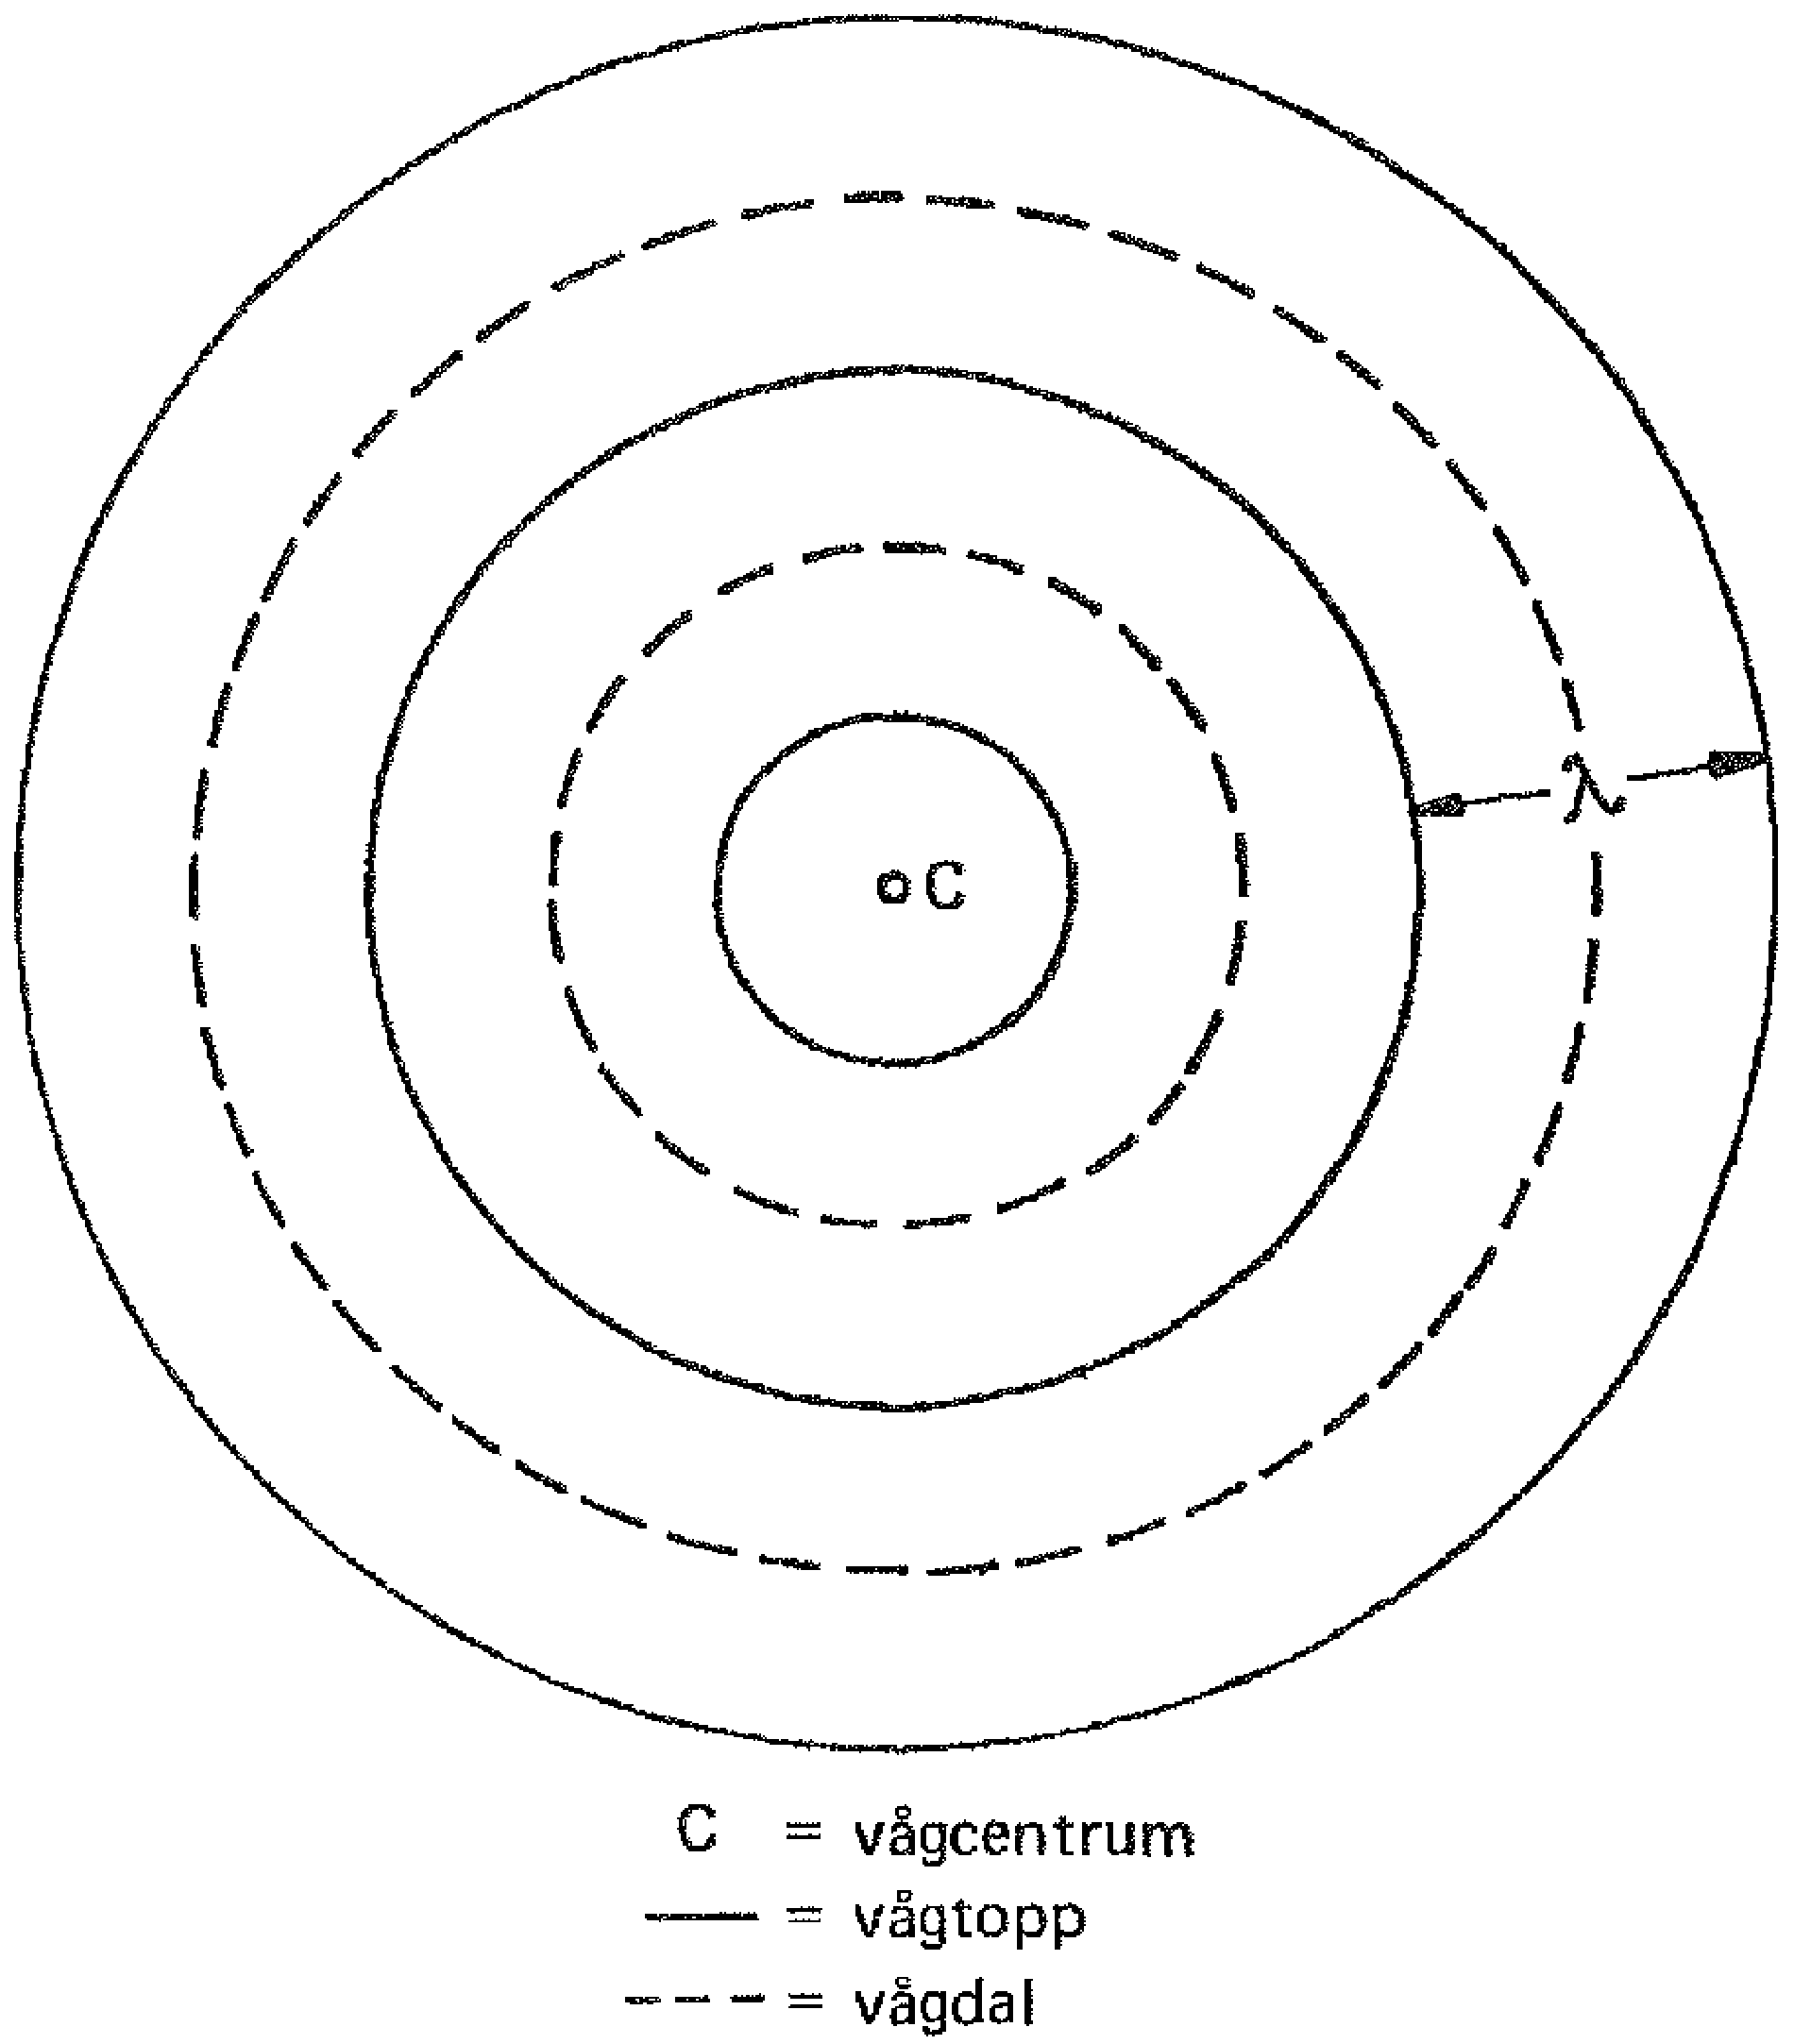
\includegraphics[width=0.5\textwidth]{images/cropped_pdfs/bild_2_1-11.pdf}
  \caption{Vågutbredning på en yta}
  \label{fig:BildII1-11}
\end{wrapfigure}

Bild \ref{fig:BildII1-10} visar vågor längs en linje.
När änden av en tråd sätts i pendling med en frekvens \(f\), så kommer till
sist hela tråden i svängning med den frekvensen.
Den pendling, som först skapades, vandrar längs tråden med
utbredningshastigheten \(v\).
Våglängden är \(\lambda\) (lambda), som är avståndet mellan två närliggande
punkter med samma svängningsläge och svängningsriktning.

\subsubsection{Vågutbredning på en yta}
\index{vågutbredningshastighet}
\index{symbol!\(v\) vågutbredningshastighet}

Bild \ref{fig:BildII1-11} visar vågutbredning på en yta.
När ett föremål släpps genom en vätskeyta, så bildas vågor som breder ut sig
som cirklar i varandra (koncentriska).

De punkter på vågen, som för ögonblicket har samma svängningsläge, och är lika
långt från energikällan, kallas för vågfront.

Sambandet mellan utbredningshastighet \(v\), våglängd \(\lambda\) och frekvens
\(f\) är

\(
\begin{array}{llll}
v = \lambda \cdot f & v \ [m/s] & \lambda \ [m] & f \ [Hz=1/s]
\end{array}
\)

Exempel: När våglängden \(\lambda = 2\ m\) och antalet svängningar per sekund
\(f = 10\ Hz\), så breder vågen ut sig med hastigheten \(v = 20\ m/s\).

\subsubsection{Vågutbredning i rummet}

\begin{wrapfigure}[12]{R}{0.5\textwidth}
  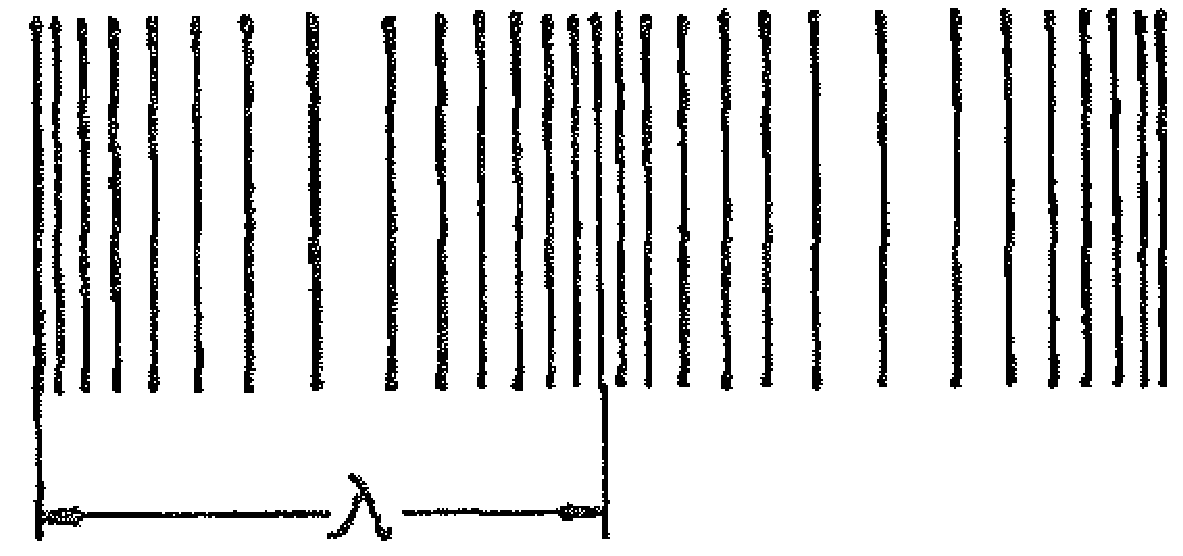
\includegraphics[width=0.5\textwidth]{images/cropped_pdfs/bild_2_1-12.pdf}
  \caption{Vågutbredning i rummet}
  \label{fig:BildII1-12}
\end{wrapfigure}

Bild \ref{fig:BildII1-12} visar vågutbredning i rummet.

Ljud är energi i form av tryckvågor i luften.
När en mekanisk kropp sätts i svängning (stämgaffel, dricksglas etc), överförs
svängningarna till den omgivande luftmassan som börjar att svänga med.
I luftmassan bildas det omväxlande över- och undertryckszoner, som breder ut
sig åt alla håll.
De mekaniska svängningarna i ljudkällan omvandlas alltså till tryckvågor.

Det mänskliga örat uppfattar tryckvågor inom frekvensområdet ca
\(15-18000\ Hz\) som ljud.
Dessa vågor kallas ljudvågor.
Utbredningshastigheten för ljudvågor är \(v = \text{ca} 340\ \text{m/s}\) vid
15~\degree C och normalt lufttryck.

\subsection{Elektromagnetiska fält}
\textbf{HAREC a.\ref{HAREC.a.1.5.2}\label{myHAREC.a.1.5.2}}
\index{elektromagnetiska fält}

Tabell \ref{tab:elektromagnetiskt_spektrum} visar elektromagnetiskt spektrum.
I detta avsnitt görs i huvudsak endast jämförelse mellan ljusvågor och
radiovågor, vilka båda är elektromagnetisk strålning.
Hur ett elektromagnetiskt fält frigörs från en ledare, framgår av kapitel
\ref{vågutbredning}.

Elektromagnetiska fält är energi, som är sammansatt av mycket snabbt svängande
elektriska och magnetiska fält.
När elektrisk ström genom en ledare ändras i styrka, så bildas ett magnetfält
omkring ledaren.
Detta magnetfält alstrar en elektromotorisk kraft (EMK), som är motriktad den
som driver fram strömmen.
Magnetfältet motverkar således strömändringen.
På liknande sätt alstrar en ändring av magnetfältet omkring ledaren en EMK i
form av ett elektriskt fält.
Detta driver en motriktad ström och därmed ett motverkande magnetiskt fält.

Både det elektriska och det magnetiska fältet har således alstrats av ändringar
i det andra och existerar därför bara tillsammans.

De båda fälten kombineras till ett elektromagnetiskt fält, som har egenskapen
att kunna stråla (breda ut sig) i alla tre dimensioner.
Beroende på frekvensen har elektromagnetiska fält olika egenskaper och
användning, vilket framgår av bilden.

\begin{table}
\begin{center}
\begin{tabular}{|rl|rl|l|}
\hline
\multicolumn{2}{|c|}{\multirow{2}{*}{Frekvens}} & \multicolumn{2}{|c|}{\multirow{2}{*}{Våglängd}} & \multicolumn{1}{|c|}{Egenskaper/} \\
 & & & & \multicolumn{1}{|c|}{användning} \\ \hline
300 & Hz  & 100 & mil & \\
  1 & kHz & 300 & km & ULF \\ \cline{5-5}
  3 & kHz & 100 & km & \\
 10 & kHz &  30 & km & VLF \\ \cline{5-5}
 30 & kHz &  10 & km & \\
100 & kHz &   3 & km & LF \\ \cline{5-5}
300 & kHz &   1 & km & \\
  1 & MHz & 300 & m & MF \\ \cline{5-5}
  3 & MHz & 100 & m & \\
 10 & MHz &  30 & m & HF \\ \cline{5-5}
 30 & MHz &  10 & m & \\
100 & MHz &   3 & m & VHF \\ \cline{5-5}
300 & MHz &   1 & m & \\
  1 & GHz & 300 & mm & UHF \\ \cline{5-5}
  3 & GHz & 100 & mm & \\
 10 & GHz &  30 & mm & SHF \\ \cline{5-5}
 30 & GHz &  10 & mm & \\
100 & GHz &   3 & mm & EHF\\ \cline{5-5}
300 & GHz &   1 & mm & \\\
  1 & THz & 300 & \(\mu\)m & Infrarött \\
  3 & THz & 100 & \(\mu\)m & ljus \\
 10 & THz &  30 & \(\mu\)m & (värme- \\
 30 & THz &  10 & \(\mu\)m & strålning) \\
100 & THz &   3 & \(\mu\)m & \\ \cline{5-5}
300 & THz &   1 & \(\mu\)m & Synligt ljus \\ \cline{5-5}
  1 & PHz & 300 & nm & \\
  3 & PHz & 100 & nm & Ultraviolett \\
 10 & PHz &  30 & nm & ljus \\ \cline{5-5}
 30 & PHz &  10 & nm & \\
100 & PHz &   3 & nm & Rönt-\\
300 & PHz &   1 & nm & gen-\\
  1 & EHz & 300 & pm & strålning\\ \cline{5-5}
  3 & EHz & 100 & pm & \\
 10 & EHz &  30 & pm & Gamma-\\
 30 & EHz &  10 & pm & strål-\\
100 & EHz &   3 & pm & ning\\
300 & EHz &   1 & pm & \\
\hline
\end{tabular}
\end{center}
\caption{Elektromagnetiskt spektrum}
\label{tab:elektromagnetiskt_spektrum}
\end{table}

\subsubsection{Ljusvågor}
\index{ljusvågor}
\index{ljushastighet}
\index{symbol!\(c\) ljushastighet i vakuum}
\index{symbol!\(\lambda\) våglängd}

Ögat uppfattar elektromagnetisk strålning bara inom ett visst frekvensområde
som ljus.
Ljusets utbredningshastighet beror av vilket material, som det passerar igenom.
I vakuum är hastigheten störst, \(c = 299\, 792\, 458\ m/s\)
(= ca \(3 \cdot 10^8\ m/s\)) \cite{SIbrochure8}.
I tätare ämnen är hastigheten lägre, t.ex. i glas ca \(200\, 000\, 000\ m/s\).
Det för människan synliga ljuset har våglängder mellan \(7,7 \cdot 10^{-7}\)
och \(3,9 \cdot 10^{-7}\ m\), motsvarande 7,7 till 3,9 tiotusendels mm.

Sambandet mellan ljusets utbredningshastighet \(c\) i vakuum, frekvensen \(f\)
och våglängden \(\lambda\) är

\(
\begin{array}{llll}
c = \lambda \cdot f & c \ [m/s] & \lambda \ [m] & f \ [Hz]
\end{array}
\)

\subsubsection{Radiovågor}
\index{radiovågor}

Även radiovågor är elektromagnetisk strålning, men inom ett lägre
frekvensområde än det för ljus.
Men utbredningshastigheten för radiovågor genom olika material följer ändå
samma lagar som de för t.ex. ljusets utbredning.

Radiovågor anses omfatta ett frekvensområde från ca 10~kHz
(\(\lambda = 30\ km\)) till 300~GHz (\(\lambda = 1\ mm\)).

Rundradio tilldelas frekvenser i intervallet 100~kHz till 1000~MHz.
Amatörradio tilldelas ett antal frekvensområden i intervallet 1,8~MHz till
250~GHz.

Att märka är att elektromagnetiska fält, som sagts ovan, förekommer så långt
ner i frekvens som ett fåtal kHz.
Detta ska självklart inte förväxlas med ljudtryck med samma frekvens.

\subsubsection{Egenskaper hos elektromagnetiska vågor}

Elektromagnetiska vågor med högre frekvens än radiovågor uppfattas som
värmestrålning, vågor med ännu högre frekvens som ljus etc., men fortfarande är
huvudegenskaperna samma.
Som exempel kan nämnas polariserade vågor.
Dessutom kan man finna motsvarigheten till sådana egenskaper som interferens,
överlagring, även i andra vågtyper, t.ex. i ljud.

\subsection{Vågpolarisation}
\textbf{HAREC a.\ref{HAREC.a.1.5.3}\label{myHAREC.a.1.5.3}}
\label{vågpolarisation}
\index{vågpolarisation}

\begin{figure}
  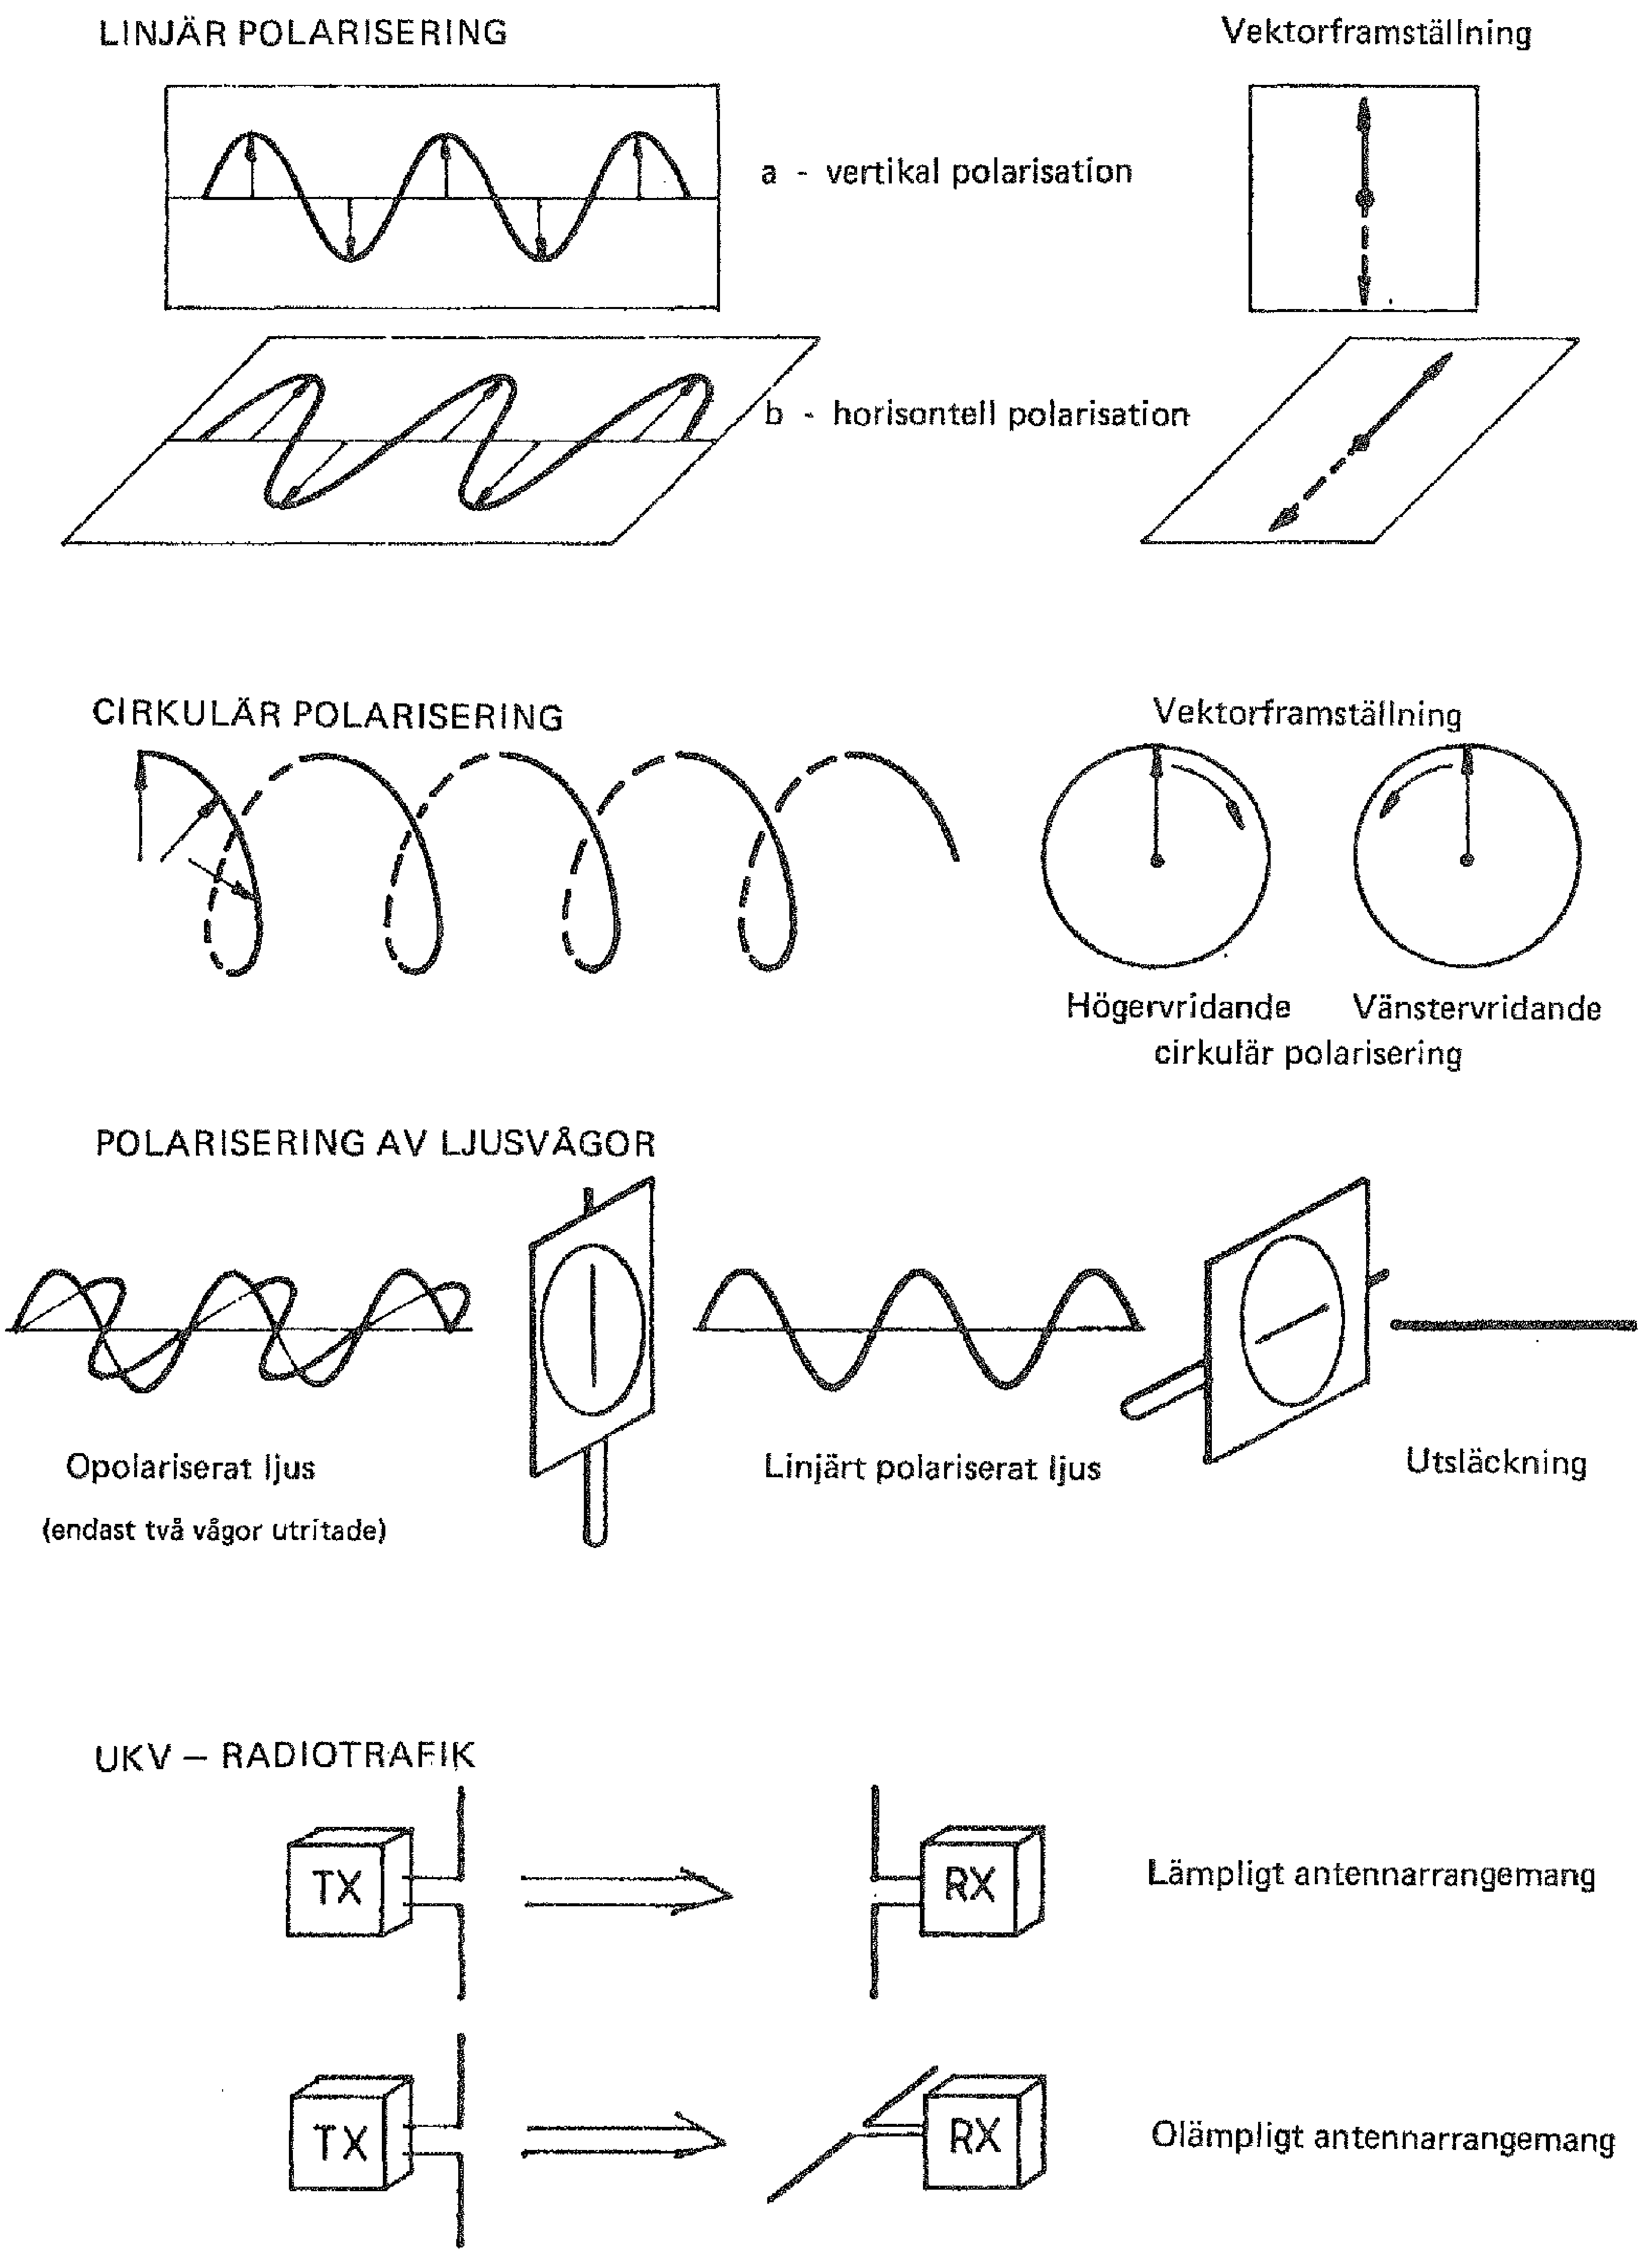
\includegraphics[width=\textwidth]{images/cropped_pdfs/bild_2_1-14.pdf}
  \caption{Polarisation av elektromagnetiska vågor}
  \label{fig:BildII1-14}
\end{figure}

Bild \ref{fig:BildII1-14} visar polarisation av elektromagnetiska vågor.

\subsubsection{Vågor längs en linje (tråd e.d.)}
En vågrörelse i ett plan kallas linjärt polariserad.
Om änden på en horisontell tråd sätts i rörelse uppåt-nedåt, uppstår på tråden
en linjärt polariserad vågrörelse i vertikalplanet -- vertikal polarisering.
Om tråden sätts i rörelse höger-vänster kommer dess svängning att vara
horisontellt polariserad.
Om tråden sätts i svängning i ett plan och detta plan ständigt vrider sig,
kommer även vågrörelsen utmed tråden att vrida sig.
En vågrörelse, vars polarisering vrider sig roterar -- kallas för cirkulärt
polariserad.
Vridning mot- respektive medurs kallas för vänster- respektive högervriden
polarisering.

\subsubsection{Elektromagnetiska vågor}

De magnetiska och elektriska fälten omkring en ledare är vinkelrätt orienterade
mot varandra.
Det elektromagnetiska fält, som de bildar tillsammans, bildar en vågfront som
är vinkelrätt orienterad mot dem.

Polariseringsriktningen för en elektromagnetisk våg definieras som den riktning
dess elektriska fält har:
\begin{itemize}
  \item vertikalt elektriskt fält -- vertikal polarisering
  \item horisontellt elektriskt fält -- horisontell polarisering.
\end{itemize}

\subsubsection{Ljusvågor}

Ljus är elektromagnetiska vågor.
När dagsljus, som f.ö. är opolariserat, belyser ett polariseringsfilter, så
passerar endast de vågkomposanter genom filtret, som har samma polarisering
som filtret.

När det polariserade ljuset därefter sänds mot ett efterföljande filter, så
passerar ljuset genom det filtret endast när det har samma polarisering som
ljuset.
När de båda filtren är vridna 90\degree~i förhållande till varandra, passerar
inget ljus alls.

\subsubsection{Radiovågor}

Radiovågor är elektromagnetiska vågor inom det frekvensområde som lämpar sig
för radiokommunikation.

Beroende på sändarantennens utformning så avger den vågor med en polarisation.
På samma sätt är en mottagarantenn mest mottaglig för vågor med en viss
polarisation.
Överföringsförlusterna blir lägst mellan antenner med samma polarisation.

I det högre frekvensområdet för radio (VHF, UHF, SHF) är polariseringsvridning
under överföringen mindre vanlig.
Genom att utforma antennerna med horisontell, vertikal eller cirkulär (höger-
alternativt vänstervriden) polarisation, så fås överföringsegenskaper för olika
syften.

Cirkulärt polariserade antenner ger lägst överföringsförluster när
polariseringsriktningen är lika i sändar- och mottagarantennen.

I det lägre frekvensområdet för radio (HF och lägre) utnyttjas oftast
rymdvågsutbredning.
Eftersom de utsända vågorna då reflekteras mot jonosfärskikt, uppstår
polariseringsvridningar som inte kan förutses.
Då är det en fördel att kunna växla mellan antenner med olika polarisation.

\subsection{Våginterferens}

\begin{figure}
  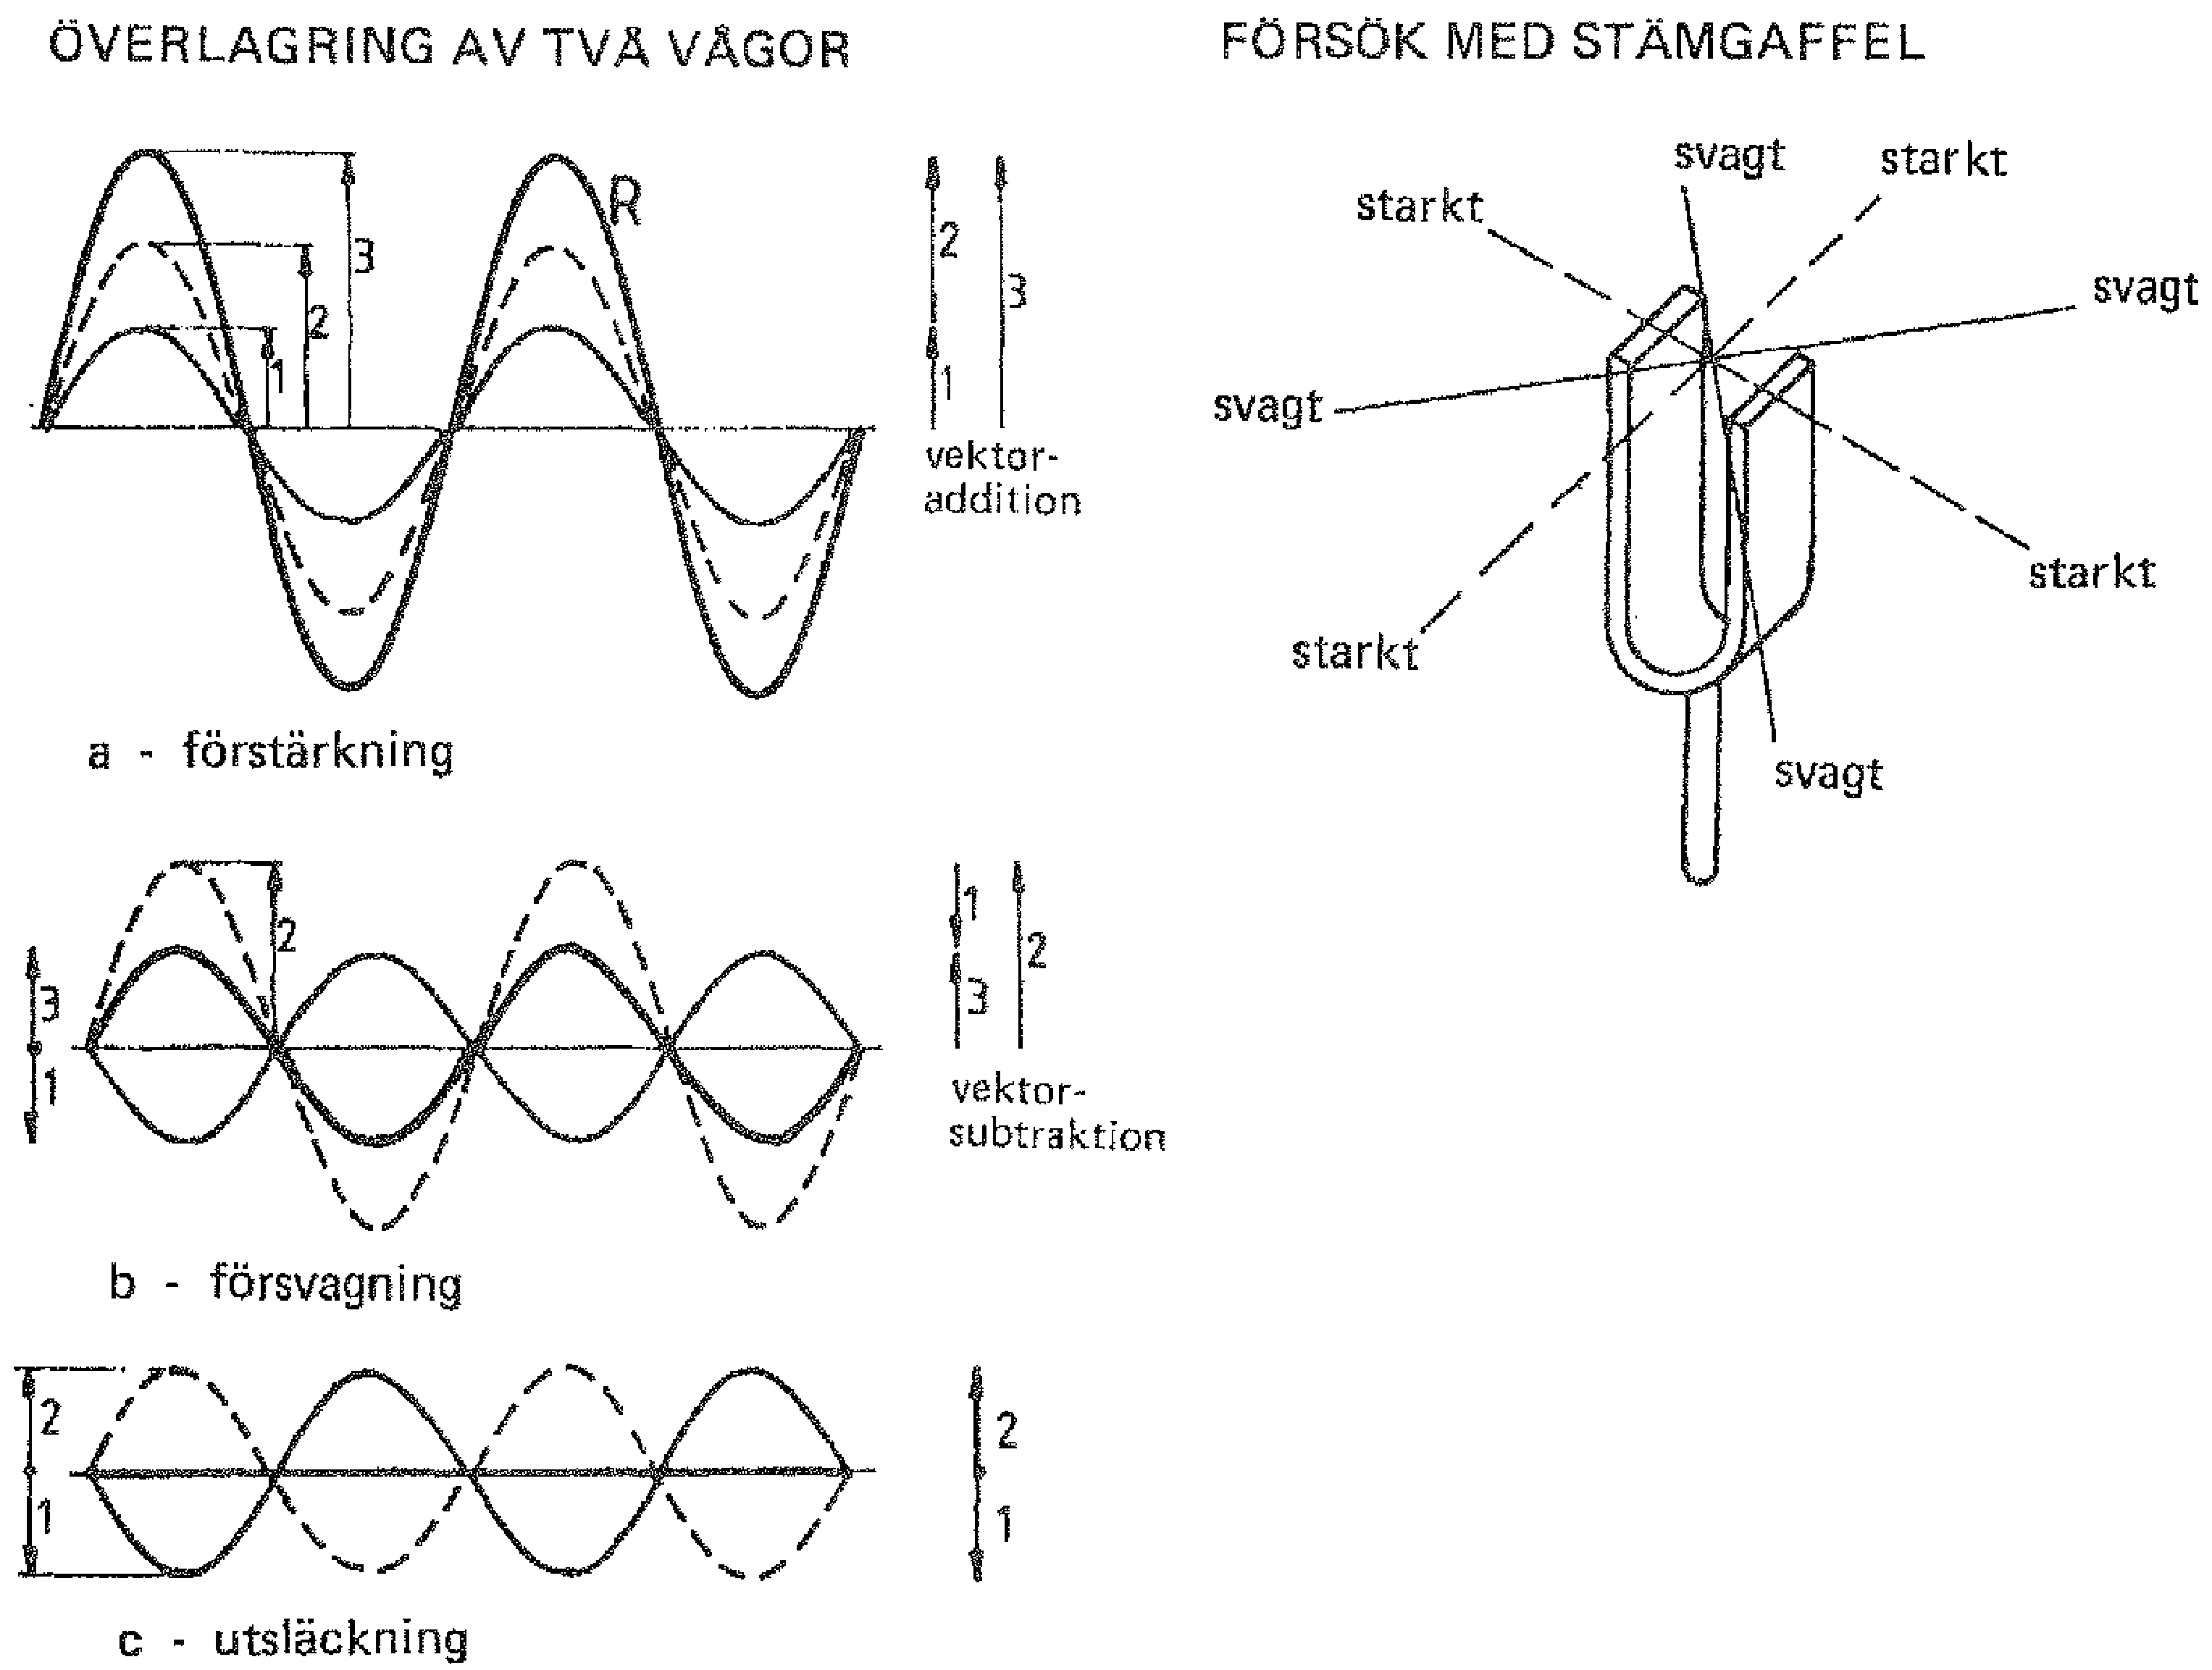
\includegraphics[width=\textwidth]{images/cropped_pdfs/bild_2_1-15.pdf}
  \caption{Våginterferens}
  \label{fig:BildII1-15}
\end{figure}

Bild \ref{fig:BildII1-15} visar våginterferens.
När vågor från olika energikällor blandas med varandra (överlagras), så kommer
de att antingen samverka eller motverka.
Beroende av det tidsmässiga läget mellan vågorna och deras amplituder, så blir
resultatet en förstärkning eller en försvagning.
Om har samma frekvens och lika stora, motriktade amplituder, så uppstår en
utsläckning, vilket kallas fädning (eng. fading).

Denna vågmekanism är liknande i gaser (luft), vätskor, elektromagnetiska fält
etc.
Ett försök kan göras med en stämgaffel som man slår an och håller intill örat.
När man vrider stämgaffeln runt sin längdaxel, så kommer avståndet mellan
vart och ett av gaffelbenen och örat att variera.
Då uppstår en växelvis med- och motverkan mellan tonerna från gaffelbenen och
därmed varierande tonstyrka.

Detta fenomen utnyttjas bl.a. i antenner för riktad sändning respektive
mottagning av radiovågor.
